% !TeX spellcheck = en_US
\section{Introduction}

Let $(x_n)_n$ be a sequence of real numbers. We say that $(x_n)_n$ is \emph{increasing} if we have $x_{n} < x_{n+1}$ for all $n \in \IN$. If we have $x_{n} \leq x_{n+1}$ for all $n \in \IN$, we say that $(x_n)_n$ is \emph{non-decreasing}. Analogously we define a \emph{decreasing} and a \emph{non-increasing} sequence. A real number is called \emph{left-computable} if there exists a computable non-decreasing (or, equivalently, increasing) sequence of rational numbers converging to it.
The left-computable numbers play an important role in computable analysis and in the theory of algorithmic randomness.

A real number $x$ is called \emph{computable} if there exists a computable sequence $(x_n)_n$ of rational numbers satisfying $\left|x - x_n\right| < 2^{-n}$ for all $n\in\IN$. It is easy to see that every computable number is left-computable, but the converse is not true. It is also easy to see that a real number~$x$ is computable if and only if there exists a computable non-decreasing sequence $(x_n)_n$ of rational numbers with $x - x_n < 2^{-n}$ for all $n \in \IN$. However, if we only require that the condition $x - x_n < 2^{-n}$ be satisfied for infinitely many $n \in \IN$, we obtain a different subset of the left-computable numbers introduced by Hertling, Hölzl, and Janicki~\cite{HHJ2023}.

\begin{defi}[Hertling, Hölzl, Janicki~\cite{HHJ2023}]
	A real number $x$ is called \emph{regainingly approximable} if there exists a computable non-decreasing sequence of rational numbers $(x_n)_n$ converging to $x$ with $x - x_n < 2^{-n}$ for infinitely many $n \in \IN$.
\end{defi}

Obviously every computable number is regainingly approximable, but the converse is not true~\cite{HHJ2023}. 
Thus, with respect to inclusion, the regainingly approximable numbers are  properly lodged between the computable and the left-computable numbers. 

For $A \subseteq \IN$, we define a real number in the interval $\left[0, 1\right]$ via $x_A := \sum_{n \in A} 2^{-(n+1)}$. Then clearly $A$ is computable if and only if $x_A$ is computable. If $A$ is only assumed to be computably enumerable, then $x_A$ is a left-computable number; the converse is not true as pointed out by Jockusch (see Soare~\cite{Soa69a}). We say that a real number $x \in \left[0,1\right]$ is \emph{strongly left-computable} if there exists a computably enumerable set $A \subseteq \IN$ with $x_A = x$.

\begin{defi}\label{def:konvergenzmodul}
	Let  $(x_n)_n$ be a convergent sequence and $x := \lim_{n\to\infty}  x_n$.
	\begin{enumerate}
		\item A function $f\colon \IN \to \IN$ is called a \emph{modulus of convergence} of $(x_n)_n$ if for all~${n \in \IN}$ and for all $m \geq f(n)$ we have $\left| x - x_m\right| < 2^{-n}$.
		\item We say that a modulus of convergence $g \colon \IN \to \IN$ of $(x_n)_n$ is \emph{optimal} if for every modulus of convergence $f \colon  \IN \to \IN$ of $(x_n)_n$ and for all $n \in \IN$ we have $f(n) \geq g(n)$.
		\item We say that the sequence $(x_n)_n$ \emph{converges computably} to $x$ if it has a computable modulus of convergence.
	\end{enumerate}
\end{defi}

\begin{figure}\label{kldhfkjradfrttsgfrtsdsf}
	\scalebox{1.02}{
		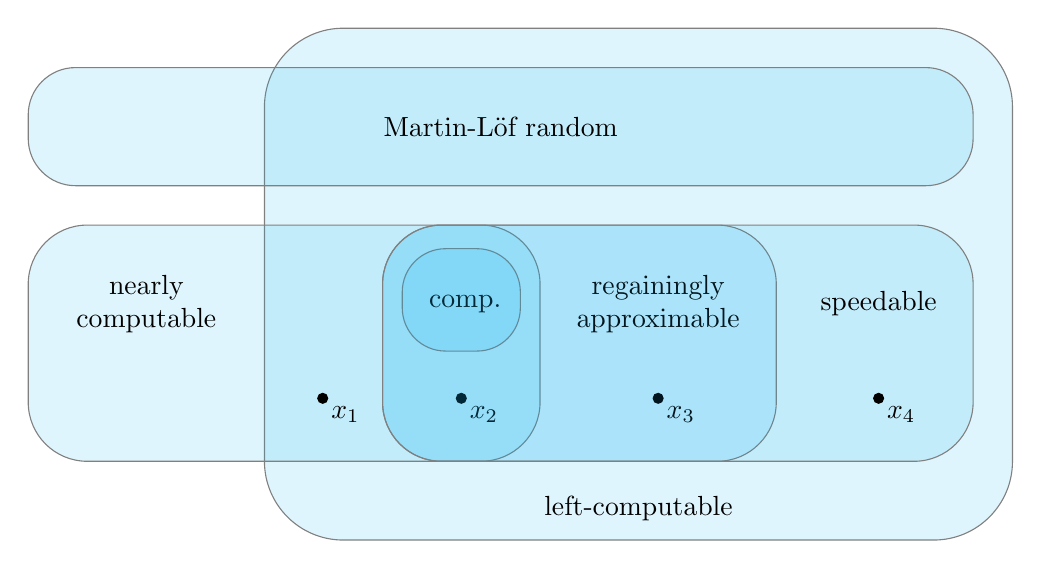
\begin{tikzpicture}[set/.style={fill=cyan,fill opacity=0.125, draw=gray},scale=2,point/.style = {circle, fill=black, inner sep=0.05cm,
				node contents={}}]
			
			% LCE
			\draw[set, rounded corners=1cm] (0, 0.25) rectangle (4.75, 3.5) {};
			\node at (2.375,0.45) {left-computable};
			
			% MLR
			\draw[set, rounded corners=0.6cm] (-1.5, 2.5) rectangle (4.5, 3.25) {};
			\node at (1.5,2.875) {Martin-Löf random};
			
			%NC
			\draw[set, rounded corners=0.75cm] (-1.5, 0.75) rectangle (1.75, 2.25) {};
			\node[align=center] at (-0.75,1.75) {nearly\\computable};
			\node at (0.37,1.15) [point=cyan, label={[label distance=-0.1cm]below right:$x_1$}];
			\draw[set, rounded corners=0.55cm] (0.875, 1.45) rectangle (1.625, 2.1) {};
			\node[align=center] at (1.25,1.75) {\phantom{.}comp.};
			\node at (1.25,1.15) [point=cyan, label={[label distance=-0.1cm]below right:$x_2$}];
			
			%reg approx
			\draw[set, rounded corners=0.75cm] (0.75, 0.75) rectangle (3.25, 2.25) {};
			\node[align=center] at (2.5,1.75) {regainingly\\approximable};
			\node at (2.5,1.15) [point=cyan, label={[label distance=-0.1cm]below right:$x_3$}];
			%speedable
			\draw[set, rounded corners=0.75cm] (0.75, 0.75) rectangle (4.5, 2.25) {};
			\node[align=center] at (3.9,1.75) {speedable};
			\node at (3.9,1.15) [point=cyan, label={[label distance=-0.1cm]below right:$x_4$}];			
	\end{tikzpicture}}
	\caption{An overview of the three different notions of benign approximability studied in this article, and of numbers witnessing their separations: $x_1$ and $x_2$ are constructed in Theorem~\ref{satz:FBNAA} and Theorem~\ref{satz:fast-berechenbar-aufholend-approximierbar}, respectively. Proposition~\ref{sadjasjhkrtjhqwejhxvbbmasdgh} establishes the existence of~$x_3$, and Corollary~\ref{dfsdjhhdbfajfkjgsdjfhdasnfbsafevcvssda} that of $x_4$.}
\end{figure}

It is clear that for every convergent sequence there exists a unique optimal modulus of convergence~$g$, but that this $g$ need  in general not be 
computable even if the sequence converges computably. It can be shown that a real number is computable if and only if there exists a computable sequence of rational numbers converging computably to it. In a detailed study, Hertling and Janicki~\cite{HJ2023} used the concept of computable convergence to define another interesting subset of the real numbers.
\begin{defi}[Hertling, Janicki~\cite{HJ2023}]\label{def:fast-berechenbar}
	\;
	\begin{enumerate}
		\item A sequence $(x_n)_n$ is called \emph{nearly computably convergent} if it converges and, for every computable increasing function $s \colon  \IN \to \IN$, the sequence $(x_{s(n+1)} - x_{s(n)})_n$ converges computably to $0$.
		\item A real number is called \emph{nearly computable} if there exists a computable sequence of rational numbers which converges nearly computably to it.
	\end{enumerate}
\end{defi}

Naturally, every computable number is nearly computable, but the converse is not true 
by a theorem of Downey and LaForte~\cite[Theorem~3]{DL02} combined with results of Stephan and Wu~\cite[Theorem~5]{SW2005} and Hertling and Janicki~\cite[Proposition~7.2]{HJ2023}.

In this article we are interested in the relationship between
the set of left-com\-pu\-table nearly computable numbers and that of regainingly approximable numbers; as every computable number is both nearly computable and regainingly approximable, we are only interested in non-computable numbers. The article consists of five sections. After discussing some preliminaries in the second section, we use the third section to
construct an example of a regainingly approximable number that is nearly computable but not computable. 
In the fourth section we give an example of a left-computable number that is nearly computable but not regainingly approximable. Both examples are built using infinite injury priority constructions.
Finally, in the fifth section, we discuss the relationship of our results to an  open problem stated by Merkle and Titov~\cite{MT2020}; they investigated when and to what extent  computable approximations to left-computable numbers can be accelerated.
\begin{defi}[Merkle, Titov \cite{MT2020}]
	A left-computable number $x$ is called \emph{speedable} if there exists a constant $\rho \in \left] 0, 1 \right[ $ and a computable increasing sequence of rational numbers $(x_n)_n$ converging to $x$ such that there are infinitely many $n \in \IN$ with $\frac{x - x_{n+1}}{x - x_n} \leq \rho$.
\end{defi}
Among other results, they gave a direct proof that speedable numbers are not Martin-Löf random\footnote{This was also  implicitly shown  by Barmpalias and Lewis-Pye~\cite[Theorem~1.7]{BLP2017}. For general background on Martin-Löf random numbers, refer to Downey and Hirschfeldt~\cite{DH2010} or Nies~\cite{Nie2009}.} and asked whether the inverse implication holds as well; that is, whether a left-computable number is speedable if and only if it is not Martin-Löf random.
Previous attempts to answer this question failed because so far speedability appears to be a notion that seems hard to work with in effective constructions. But as it turns out, regaining approximability is the key to approaching the problem. Namely, we prove that the concepts of speedable and regainingly approximable numbers are equivalent within the nearly computable numbers; thus, together with the construction of the fourth section, we obtain a negative answer to the open question, our final main result.
Figure~\ref{kldhfkjradfrttsgfrtsdsf} provides an overview of the relationship of the different classes of numbers studied in this article.





